\documentclass[11pt, a4paper]{scrartcl}
\usepackage[utf8]{inputenc}
\usepackage[ngerman]{babel}
\usepackage[dvipsnames]{xcolor}
\usepackage{amsmath}
\usepackage{amssymb}
\usepackage{enumitem}
\usepackage{hyperref}
\usepackage{minted}
\usepackage[fencedCode]{markdown}
\usepackage{graphicx}
\graphicspath{{images/}}


\title{Embedded Systems}
\author{Zusammenfassung}
\date{Wise24/25}

\begin{document}

\maketitle

\tableofcontents
\newpage


% --- START DES EIGENTLICHEN INHALTS -------------------------------------------------

\raggedright
\section{I/O Ports}

Ports werden durch 8 Bit Register konfiguriert.

\textbf{D}ata \textbf{D}irection \textbf{R}egister (DDR) \\

\vspace{0.5em} 

0 = Input 

1 = Output

\vspace{1em} 

\textbf{Default} Wert ist \textbf{0} bzw. \textbf{Input}.
Damit wird verhindert, dass ein Verbraucher ausversehen zu viel Strom zieht und damit den Mikrocontroller beschädigt.  

\vspace{2em} 

\subsection{DDRn}

DDRB - Port B Data Direction Register

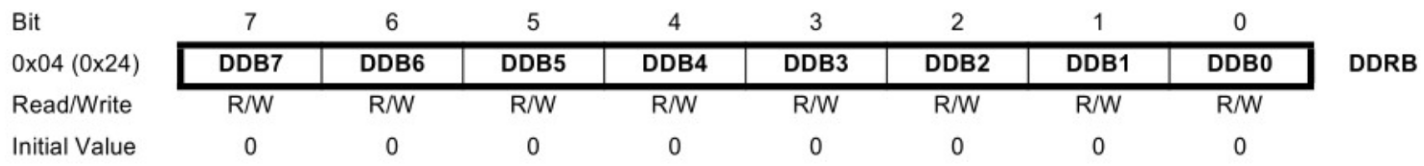
\includegraphics[width=1\textwidth]{01/01.png}

\vspace{2em} 

$\rightarrow$ \textbf{DDRn} Register legt die Richtung fest (Input oder Output)!

\newpage 




\subsection{Digitale Outports}

Wurde ein Pin als Output definiert, so kann man ihn über das \textbf{PORTn} Register steuern.

\subsubsection{PORTn}

PORTB - Port B Data Register

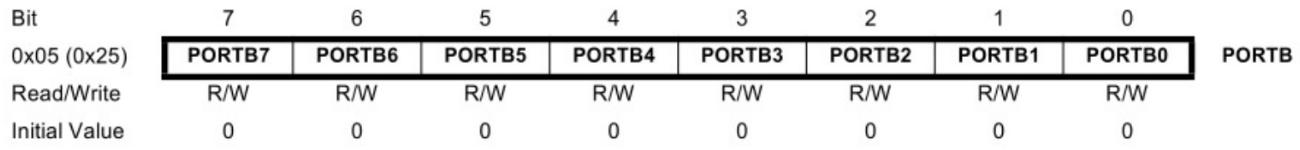
\includegraphics[width=1\textwidth]{01/02.png}

\vspace{2em} 

$\rightarrow$ \textbf{PORTn} Register definiert, ob Output high oder low!

\vspace{3em} 

Beispiel: High Pegel auf PORTB3

\markdownInput{markdown/01/01.md}

Hinter \textbf{DDB3} und \textbf{PORTB3} steckt nur eine Zahl, um die eine 1 nach links verschoben wird im Register.

\newpage



\subsection{Digitale Inports}

Wurde ein Pin als Input in DDRn definiert, so kann man ihn über das \textbf{PINn} Register abfragen.

\subsubsection{PINn}

PINB - Port B Input Pins Address

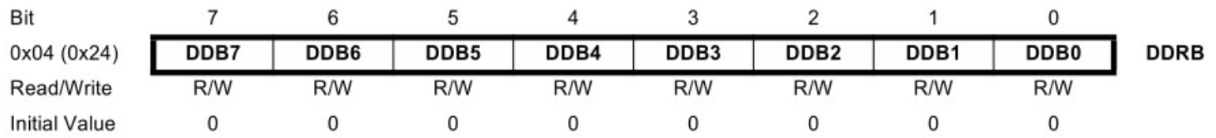
\includegraphics[width=1\textwidth]{01/03.png}

\vspace{2em} 

Beispiel: Pin 3 von DDRB auslesen

\markdownInput{markdown/01/02.md}

\vspace{1em} 

ATmega328p hat bei allen Ports einen interenen Pull-Up Widerstand!

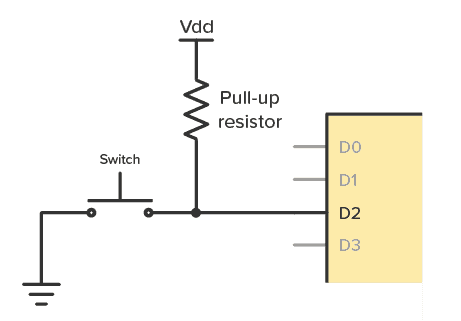
\includegraphics[width=0.4\textwidth]{01/04.png} 

Taster brückt auf Masse! Deshalb wird im Code nach 0 abfragen!

\vspace{1em}

\newpage




\end{document}
